\documentclass[a4paper,jou,natbib,floatsintext,donotrepeattitle]{apa6}

\usepackage[english]{babel}
\usepackage[utf8x]{inputenc}
\usepackage{amsmath}
\usepackage{graphicx}
\usepackage[colorinlistoftodos]{todonotes}
\usepackage{xcolor}
\usepackage[draft,inline,nomargin,index]{fixme}
\usepackage[hidelinks]{hyperref}
\usepackage{verbatim}
\usepackage{nameref}
\usepackage{booktabs}
\usepackage{lineno}
\usepackage{amsfonts}
\usepackage{booktabs}
\usepackage{siunitx}
\usepackage{minted}
\usepackage[symbol]{footmisc}
\usepackage{listings}
\usepackage{filecontents}
\usepackage{multicol}
\usepackage{svg}
\usepackage[sfdefault,condensed]{roboto} %% Option 'sfdefault' only if the base font of the document is to be sans serif
\usepackage[T1]{fontenc}
\usepackage{stfloats}

\usepackage{graphicx} % resize tables

\usemintedstyle{monokai}
\definecolor{bg}{HTML}{282828} % from https://github.com/kevinsawicki/monokai

\fxsetup{theme=color,mode=multiuser}
\FXRegisterAuthor{ab}{sab}{\color{blue}A} % abnote{} with text inside to edit
\FXRegisterAuthor{bb}{sbb}{\color{purple}B} % bbnote{} with text inside to edit
\FXRegisterAuthor{ln}{sln}{\color{violet}L} % lnnote{} with text inside to edit

% adapting dois to follow APA6
\renewcommand{\doiprefix}{}
\newcommand{\doi}[1]{\href{https://doi.org/#1}{https://doi.org/#1}}

% making footnotes in arabic style
\renewcommand{\thefootnote}{\arabic{footnote}}
\interfootnotelinepenalty=10000

% enabling lines number
\linenumbers

%\fxsetup{theme=color,mode=multiuser}
%\FXRegisterAuthor{ab}{sab}{\color{blue}Amelie} % abnote{} with text inside to edit
%\FXRegisterAuthor{bb}{sbb}{\color{purple}Brice} % bbnote{} with text inside to edit
%\FXRegisterAuthor{ln}{sln}{\color{violet}Lad} % lnnote{} with text inside to edit

\title{A fully automated, transparent, reproducible, and blind protocol for sequential analyses}

\shorttitle{Automated sequential analyses}
\twoauthors{Brice Beffara-Bret \qquad Amélie Beffara-Bret}{Ladislas Nalborczyk}
\twoaffiliations{LPPL - EA 4638, Université de Nantes, Nantes, France \\ The Walden III Slowpen Science Laboratory, Villeurbanne, France}{Department of Experimental Clinical and Health Psychology, Ghent University, Belgium \\ The Walden III Slowpen Science Laboratory, Villeurbanne, France}

\abstract{Despite many cultural, methodological and technical improvements, one of the major obstacle to results reproducibility remains the pervasive low statistical power. In response to this problem, a lot of attention has recently been drawn to sequential analyses. This type of procedure has been shown to be more efficient (to require less observations and therefore less resources) than classical fixed-N procedures. However, these procedures are submitted to both intrapersonal and interpersonal biases during data collection and data analysis. In this tutorial, we explain how automation can be used to prevent these biases. We show how to synchronise open and free experiment software programs with the Open Science Framework and how to automate sequential data analyses in R. This tutorial is intended to researchers with beginner experience with R but no previous experience with sequential analyses is required.}

\keywords{sequential analysis, sequential testing, sequential Bayes factor, automation, expectancy effects, reproducibility, blind analyses}

\note{\vspace{0.1cm}\footnotesize{Under peer review at Meta-Psychology. Editorial process can be accessed at: \href{https://osf.io/v2pnc}{\protect \nolinkurl{https://osf.io/v2pnc}}. \par Anyone can contribute with Open Peer Review. Contact the editor at \href{mailto:rickard.carlsson@lnu.se}{\nolinkurl{rickard.carlsson@lnu.se}}, \par or contribute directly in the OSF project.\par \textcolor{red}{This manuscript has not yet been published. Cite at your own risk.}\par}}

\authornote{Correspondence concerning this article should be addressed to Brice Beffara-Bret, Université de Nantes, Nantes, France. \\E-mail: \href{mailto:brice.beffara@univ-nantes.fr}{\nolinkurl{brice.beffara@univ-nantes.fr}} }

\begin{document}

% defining a new command for counting words
\newcommand{\quickwordcount}{
  \immediate\write18{texcount -1 -sum -merge main.tex > \jobname-words.sum}
  \input{\jobname-words.sum}words
}

\maketitle

Wordcount: This document contains \textbf{\quickwordcount}.

\newpage

%%%%%%%%%%%%%%%%%%%%%%%%%%%%%%%%%%%%%%%%%%%%%%%%%%%%%%%%%%%
% table of contents (to be removed upon submission)
%%%%%%%%%%%%%%%%%%%%%%%%%%%%%%%%%%%%%%%%%%%%%%%%%%%%%%
% \tableofcontents
% \newpage
%%%%%%%%%%%%%%%%%%%%%%%%%%%%%%%%%%%%%%%%%%%%%

\section{On reproducibility}

It may be referred to as a \textit{crisis}, a \textit{revolution}, or a \textit{renaissance}, but Psychology has undeniably known a decade of unparalleled methodological reflection and reform \citep[for an overview, see][]{nelson_psychologys_2018,fidler_reproducibility_2018}. Although many of the practices that are currently recognised as part of the problem (e.g., poor understanding of statistical methods, questionable research practices) have long been acknowledged \citep[e.g.,][]{babbage_reflections_1830},\footnote{Where the same could be said for recently proposed solutions like preregistration or radical transparency \citep[e.g.,][]{de_groot_meaning_2014}.} recently introduced practices have brought considerable improvements to the \textit{reliability} of findings in psychological science \citep[e.g., see][]{smaldino_open_2019}.

There are many ways to define what reproducibility is, and it is often unclear what is meant by the terms of reproducibility, replicability, repeatability, or reliability. To avoid these confusions, we adopt the terminology suggested by \cite{goodman_what_2016}. When discussing research reproducibility, we make a distinction between i) methods reproducibility: the ability to reproduce, as closely as possible, the methodological procedures developed by a certain team (i.e., what is usually meant by \textit{reproducibility}), ii) results reproducibility: the ability to reproduce a certain result in a given methodological settings (i.e., what is usually meant by \textit{replicability}), and iii) inferential reproducibility: the ability (for an independent team) to replicate an inferential conclusion, that is, to arrive at the same conclusion.

Whereas results reproducibility concerns the outcome of a computational or experimental procedure, methods reproducibility is a property of the methods being used to produce this particular outcome. As put by \cite{meehl_appraising_1990}, a scientific study is akin to a recipe, and a good methods description should allow other cooks to prepare the same kind of cake as the person that wrote the recipe did. As such, methods reproducibility is essential to results reproducibility. Fortunately, recent technical developments have made the task far easier than it used to be. Key components of a modern reproducible workflow may include:

\begin{itemize}
  \item Transparency: exhaustive and intelligible description and sharing of all materials, scripts, etc. \citep[for a practical introduction, see][]{klein_practical_2018}
  \item Self-containment: writing reproducible documents in LaTeX or RMarkdown \citep[e.g., see the \texttt{R} package \texttt{papaja,}][]{Aust_papaja_2018} and sharing self-contained code (e.g., see https://codeocean.com)
  \item Version control: using Git and Github (or Gitlab) to track changes in working documents \citep[for an introduction, see][]{vuorre_curating_2018}
  \item Automation: minimising mistakes by automatising as many steps of the research process as possible \citep[e.g.,][]{rouder_what_2016, rouder_minimizing_2018,yarkoni_enhancing_2019}
\end{itemize}

Although methods reproducibility is essential to results reproducibility, it is not sufficient. Despite having a long history of scrutiny in Psychology, one of the major threats to results reproducibility remains statistical power, where power can be broadly defined as the probability of achieving a certain goal, given that a suspected underlying state of the world is true \citep{kruschke_doing_2015}. We know that a low powered result has (all other things being equal) a lower probability to replicate, the initial result being attached with a higher probability of erroneous inference \citep[e.g.,  type-M or type-S errors,][]{gelman_beyond_2014}. Even though there are many ways to increase statistical power \citep[e.g., see][]{hansen_seven_1994}, we focus here on \textit{sequential testing}, that is, the continuous analysis of data during its collection. This procedure has been shown to \textit{optimise} the amount of resources (e.g., money and time) to be spent in order to attain a certain goal, as compared to classical a priori power analyses strategies \citep{lakens_performing_2014,schonbrodt_sequential_2017}.

We turn now to a brief presentation of several sequential analyses procedures, followed by a discussion of the methodological precautions that need to be undertaken to ensure the validity of these procedures. Finally, we outline the core aspects of a "born-open" \citep[following the terminology of][]{rouder_what_2016}, fully automated and reproducible workflow for sequential analyses.

\section{A brief introduction to sequential analyses procedures}

%\cite{edwards_bayesian_1963} famously stated: "the rules governing when data collection stops are irrelevant to data interpretation. It is entirely appropriate to collect data until a point has been proven or disproven, or until the data collector runs out of time, money, or patience". Whereas the Bayesian perspective is generally in agreement with this position \citep[e.g.,][]{rouder_optional_2014}, it might also be contested from a statistical error  perspective \citep[e.g., see][]{mayo_statistical_2018}. In the latter approach, the consistency of derived error probabilities is crucially dependent on  sampling intentions (and realisation), which are as such legitimately allowed to enter the inference. Thus, performing sequential testing in the frequentist framework requires particular adjustments to preserve the error rates (and the severity) of the test that is conducted sequentially \citep[for an overview, see][]{lakens_performing_2014}. In this tutorial we discuss Bayesian sequential analyses. However, the recommendations we provide also apply to frequentist sequential analyses.

In this section, we briefly introduce three sequential analysis procedures that address three distinct goals. More precisely, these procedures permit to either i) accumulate relative evidence for a hypothesis (the \textit{sequential bayes factor} procedure) or ii) efficiently accept or reject a value or range of values for a parameter (the sequential HDI+ROPE procedure) or iii) sample observations until a desired level of estimation precision is reached.

\subsection{Sequential Bayes factor}

\cite{schonbrodt_sequential_2017} presented an alternative to null-hypothesis significance testing with a priori power analysis (NHST-PA) by introducing the \textit{Sequential Bayes Factor} (SBF) procedure. The SBF procedure uses Bayes factors (BFs) to iteratively examine the relative evidential support for a hypothesis during data collection.\footnote{Technically speaking, the Bayes factor is a ratio of marginal likelihoods (i.e., what is considered as \textit{evidence} in the Bayesian framework). Broadly, a BF can be interpreted as an updating factor, indicating how credibility should be re-allocated from prior knowledge (what was known before seeing the data) to posterior knowledge (what is known after seeing the data).} The first step of the SBF procedure is to pick thresholds (one for each of the two hypotheses being compared) that determine the end of data collection. These thresholds should be selected to reflect the level of evidence that the experimenter consider sufficient to stop data collection, but should also be defined in consideration of specific goals and costs-benefits analyses. Indeed, more stringent thresholds require larger sample sizes, but are associated with lower risks of misleading inferences (false positive and false negative), all other things being equal. Then, after picking the appropriate prior distribution for the alternative hypothesis, a first batch of observations is collected, during which no BF is computed (to avoid misleading inferences due to early terminations). Starting at $n_{min}$ observations (the a priori defined minimum sample size), a BF is computed at each stage (or each observation). The sampling procedure goes on until the current BF reaches the a priori defined threshold or until reaching $n_{max}$ observations (the a priori defined maximum sample size).

%likelihood ratio tests allowing to evaluate whether collected data are more in support of one hypothesis or another. A BF can be expressed as the ratio of two probabilities. These probabilities are the probability of the data given each hypothesis. The $BF_{10}$ is the ratio between the probability of data given the $H_1$ hypothesis and the probability of data given the $H_0$ hypothesis. $BF_{10} = 7$ means that data is 7 times more probable under $H_1$ than under $H_0$. A BF can therefore be in favour of $H_1$ (conventionally from $BF_{10} > 3$), in favour of $H_0$ (conventionally from $BF_{10} < 1/3$), or rather indecisive (conventionally $1/3 < BF_{10} < 3$).

\cite{schonbrodt_sequential_2017} provided detailed simulation results of this procedure when comparing the means of two independent groups (the equivalent of a two-samples t-test). They show that the error rates and the average length of the procedure (i.e., how many observations are needed to reach the threshold) are a function of both the population effect size, the threshold, and the prior for the alternative hypothesis. For instance, when chasing a medium effect size (d = 0.5) and when using a "medium scaled" prior for the alternative (r = 1), stopping data collection at $BF = 6$ instead of $BF = 3$ results in a percentage of wrong inferences of 4.6\% instead of 40\% \citep[see Table 1 in][p. 10]{schonbrodt_sequential_2017}.

Based on these results, it is possible to combine prior guesses or expectations with the known properties of the SBF procedure to design experiments. This strategy is known as \textit{design analysis} and includes the classical power analyses of the NHST framework as a particular case. In this vein, Schönbrodt \& Wagenmakers (2018) introduced the \textit{Bayes Factor Design Analysis} tool and demonstrated how this strategy can help to design more informative empirical studies (see also Stefan, Gronau, Schönbrodt, \& Wagenmakers, 2019).

%, i.e. BF values which enough evidence for a defined goal. These thresholds will the limit which, when reached, will indicate that data collection can be stopped. For instance, one can decide to set a threshold at $BF_{10} = 10$ for $H_1$ and $BF_{10} = 1/7$ for $H_0$. This means that data collection will stop when the $BF_{10}$ reach 10 or a higher value, or when the $BF_{10}$ reach 1/7 or a lower value.

 %To sum up, the SBF procedure allows for iterative data collection up until a predefined level of evidence and does not suffer from the pitfalls associated with NHST-PA. Testing mean differences between two independent groups, \cite{schonbrodt_sequential_2017} shows that the SBF design typically needs 50\% to 70\% smaller samples to reach a conclusion about the presence of an effect, as compared with optimal NHST-PA (where \textit{optimal} stands for an idealised situation in which the a priori targeted effect would be exactly equal to the population effect size), with both analyses showing similar long-term error rates.

\subsection{The sequential HDI+ROPE procedure}

Bayes factors are not the only available option to perform sequential testing. Whereas BFs quantify the evidence in favour of an hypothesis (relative to another hypothesis), each individual hypothesis can also be examined on its own. For instance, the hypothesis that the group difference of some measured variable is equal to zero might be assessed by looking directly at the posterior distribution of the group difference.\footnote{The posterior distribution is the result of any Bayesian analysis. It is a probability distribution that allocates probability to parameter values, given the model (including the priors) and the observed data.} This distribution can be summarised via its mean and \textit{highest density interval} (HDI), an interval that contains the X\% most credible values for the parameter \citep{kruschke_bayesian_2018-1}.\footnote{The HDI is a particular type of credible interval, the Bayesian equivalent of the frequentist confidence interval. It should be noted however that the interpretation of Bayesian and frequentist intervals differ considerably \citep[e.g.,][]{morey_fallacy_2016, nalborczyk_pragmatism_2019}.} The hypothesis according to which the group difference is equal to zero can then be assessed by checking whether the HDI includes zero as a credible value. Alternatively, and more interestingly, the HDI can be compared to a \textit{region of practical equivalence} \citep[ROPE,][]{kruschke_rejecting_2018}, defining the range of effect sizes that we consider as negligible (i.e., equivalent to zero) for practical purposes.

The comparison of  HDI and ROPE can be summarised by computing the proportion of the HDI that is included in the ROPE, giving an idea of the extent to which the hypothesis of no effect is supported. Alternatively, the comparison of the HDI to the ROPE can result in three categorical outcomes: i) the null hypothesis is rejected (when the HDI falls \textit{completely} outside the ROPE), ii) the null hypothesis is accepted (when the HDI falls \textit{completely} inside the ROPE), or iii) the data is said to be inconclusive (when neither of the above applies).

When the goal of the analysis is to accept or reject a reference value, it is then possible to stop data collection when the HDI does not include this reference value. Thus, this procedure is similar to the SBF procedure, except that the sampling procedure is terminated by a (conclusive) comparison of a HDI to a ROPE, instead of being terminated by a comparison of a BF value to some threshold \citep[for a detailed study of the characteristics of this procedure, see][]{kruschke_doing_2015}.

\subsection{Aiming for precision}

Because data collection stops when the accumulated evidence reaches a certain threshold, sequential hypothesis testing procedures (e.g., SBF or HDI+ROPE) are known to be biased by extreme observations. In other words, the data collection stops when the collected data supports the hypothesis, preventing the opportunity of collecting contradictory data afterwards \citep{kruschke_doing_2015}. Performing sequential analysis until a certain estimation precision is reached overcomes this bias \citep{kruschke_doing_2015}. In this procedure, the goal is not to stop data analysis based on the rejection of an hypothesis but rather to sample observations until a predefined level of precision in a parameter (including effect size) estimation is reached. The estimation precision can be quantified by the width of the HDI and \cite{kruschke_doing_2015} proposes to stop data analysis when the HDI width is less than 80\% of the ROPE's width. For instance, if the \textit{smallest effect size of interest} \citep[SESOI,][]{lakens_equivalence_2018} is $\delta = 0.2$, we can define a ROPE around 0 from $\delta = -0.1$ to $\delta = 0.1$. This means that we will consider an effect as approximately null when it is less than half our SESOI. Planing for precision, we would therefore stop data collection when the width of our HDI (on the estimate of the effect size) is inferior to $0.8 \times 0.2 = 0.16$ \citep{kruschke_rejecting_2018}. \par

Of course, there are other methods to determine the desired level of precision. For instance, researchers can base their SESOI on an effect of minimal clinical relevance. In this context, the SESOI varies depending on the costs and benefits of the treatment \citep{lakens_equivalence_2018}. We can also imagine other criteria to determine precision on the basis of the ROPE. In any case, even if one wants to check whether the HDI falls inside the ROPE at the end of data collection, planing for precision enables us to focus on parameter or effect size estimation instead of hypothesis testing. If we decide to plan for moderate precision, we will not need a large amount of observations, but it is likely that the HDI will overlap the ROPE. As a consequence, it will not be possible to reach a categorical conclusion. If we plan for high precision, more observations will be needed to stop data collection, but hypothesis testing will be improved as well as precision. In most situations, planing for precision will require more observations than hypothesis testing. \par

Whatever the procedure, the stopping rule should be thought carefully by considering and balancing the costs and benefits of collecting more observations. A small number of observations is affordable but likely to lead to biased conclusions. A large number of observations can be expensive but likely to lead to more robust conclusions. Both frequentist and Bayesian methods have their ways to deal with risks and errors in sequential hypothesis testing. Criteria are modified for sequential hypothesis testing so that "significant" p-values (e.g., .0294 instead of .05 for one interim analysis, \citealt{lakens_performing_2014}) or Bayes factors (e.g., BF = 6 instead of BF = 3 depending on acceptable error rates, \citealt{schonbrodt_sequential_2017}) are not the same as classical (non sequential) hypothesis testing. This should also be considered in sequential the HDI+ROPE procedure.

% before to turn to a discussion of the potential limitations of these procedures. Finally, we provide practical recommendations to limit these potential biases during sequential analyses...

\subsection{Some difficulties}

The procedures previously described and discussed in \cite{schonbrodt_sequential_2017} and \cite{kruschke_doing_2015,kruschke_rejecting_2018} offer an attractive perspective on data collection. However, some precautions need to be undertaken in order to preserve a good precision or the long-term error rates they provide. More precisely, we discuss two main categories of biases that need to be controlled. We call the first category of biases \textit{intrapersonal biases}, as biases that are expressed \textit{within} individuals. These biases mainly emerge during data analysis and data reporting. We call the second category of biases \textit{interpersonal biases}, as biases that are expressed \textit{between} individuals. These biases mainly emerge during data collection (e.g., when the researcher interacts with participants). \par

These biases can arise in any study but sequential procedures present specific risks on both the intra and interpersonal dimensions. We explain why in the next section.

\section{What could possibly go wrong?}

\subsection{Intrapersonal biases during sequential analyses}% (or Researcher degrees of freedom in data analysis)}

Most intrapersonal biases occur because of what some would call the "researcher degrees of freedom" \citep{simmons_false-positive_2011,wicherts_degrees_2016-1}. Following \cite{wicherts_degrees_2016-1}' nomenclature, we identified the following intrapersonal biases as having increased risks in sequential procedures: 

\begin{itemize}
    \item \textbf{C3}: Correcting, coding, or discarding data during data collection in a non-blinded manner.
    \item \textbf{A1}: Choosing between different options of dealing with incomplete or missing data on ad hoc grounds.
    \item \textbf{A2}: Specifying pre-processing of data (e.g., cleaning, normalization, smoothing, motion correction) in an ad hoc manner.
    \item \textbf{A3}: Deciding how to deal with violations of statistical assumptions in an ad hoc manner.
    \item \textbf{A4}: Deciding on how to deal with outliers in an ad hoc manner.
\end{itemize}

These degrees of freedom allow flexibility when processing data before statistical inference. This flexibility can be dangerous when incentives, cultural norms, or previous practices  influence data analysis, and where there are few safeguards. Thus, the intrapersonal nature of these biases does not refer to an absence of social influence, but rather to biases occurring at the point where the researcher makes choices on her own. This can be the case when someone discards an outlier to reach a significant result because it is easier to publish with significant results. This can also be the case when one tries different data transformations to best match their preferred hypothesis. Here the problematic nature of the degrees of freedom is the researcher's subjectivity. Discarding an outlier or transforming data is not necessarily the result of being an outlier or being skewed data, but can also be the result of what the researcher wants to see because of economic, social (e.g., reputation pressure), cultural contexts. These biases are not specific to sequential procedures but their consequences might be amplified during sequential procedures because of the possible impact of each look at the data. Indeed, the degrees of freedom can impact data analysis at time t1 which can in turn impact data collection in a self-perpetuating cycle. Data analysis at time t2 is therefore likely to be biased by the degrees of freedom at time t2 but also at time t1. Thus, errors accumulate because the effects of the degrees of freedom are multiplied. \par

When a data analyst has expectations about what should be observed, the data analysis is likely to be biased by these expectations through confirmation (favouring an hypothesis) or disconfirmation (stronger scepticism toward data against the hypothesis than toward data corroborating the hypothesis) biases \citep{lilienfeld_blind_2017}. While continuously analysing data, the data analyst is faced with many choices about the best way to deal with incoming data. Based on previous studies, they might have expectations about the range of plausible values, or they might need to use particular methods to process physiological signals, to recode or to transform data in a specific way, and so on. We urge researchers to make these decisions explicit before data collection. \par

The properties of sequential procedures have been studied extensively via simulation \citep{schonbrodt_sequential_2017,wagenmakers_bayesian_2017,kruschke_doing_2015}. However, noise and irregularities in simulated data only come from sampling variability, and not from practical problems that can be encountered during empirical data collection (e.g., technical issues or experimenter biases). When collecting data, researchers would like to get as close as possible to the shape of simulated data (i.e., we would like to minimise other sources of errors than sampling variability). In order for the BF, the HDI or the precision to be reliable stopping criteria, they have to be computed on reliable data. We acknowledge that what can be considered as \textit{reliable} data heavily depends on the type of study. As such, decisions concerning the analysis workflow should be justified by the existing literature as much as possible. However, changing the criterion and methods for data preparation based on the state of the sequential procedure is not acceptable. The result of an experiment cannot determine the way it is itself defined. Real-time result-hacking would jeopardise the confidence one can have in this result. \par

Therefore, we propose that all the steps of the sequential procedure (i.e., data preparation and cleaning, outliers detection, data transformation, model assumptions checks, and data analysis) should be automated and performed in an incremental manner. The entire dataset can be continually reanalysed, including former outliers, so that the process  follows the progressive incorporation of new observations. Put more formally, such a procedure should be able to take into account that an extreme observation at time \textit{t} might not be extreme anymore at time \textit{t+n} (and should therefore be \textit{re-included} in subsequent analyses).

The fact that this iterative procedure is automated should prevent the data analyst from the hazards that are commonly encountered during data manipulation (see previous section). These hazards have particularly important consequences in sequential procedures in comparison to traditional (i.e. fixed-n) procedures because of the incremental nature of evidence accumulation. A specific preprocessing choice at time \textit{t} can influence inference criteria computation at time \textit{t+n} which can subsequently influence another preprocessing choices and so on. With accumulated modifications in preprocessing decisions, the inference criteria are not only computed based on data but also on sequential and incremental choices from the scientist. We propose that these steps could instead be programmed and coded on the basis of preregistered choices, before starting to collect data. Preregistered automated data analysis would therefore ensure conclusions based on empirical procedures to be similar to the results (e.g., long-term error rates) provided by \cite{schonbrodt_sequential_2017} or \cite{kruschke_doing_2015} using simulation, and explicitly fulfil the requirements of transparency and reproducibility. \par

However, being able to define in advance the goal and the criteria for success of these sequential procedures requires i) to be well aware of the literature of interest, ii) to know how data behave by manipulating data from very similar previous experiments or pre-tests, iii) to be able to implement a procedure of data preparation for model computation before seeing new data. These three points might seem trivial but are even more important for sequential analyses than classical procedures in order to avoid intermediate influences in data preparation based on known interim results. \par

In addition to these intermediate influences (i.e., influences between the collection of the first batch of data and the final data analysis) in data preparation, intermediate influences can also be problematic during data collection. These influences are what we call "interpersonal biases".

\subsection{Interpersonal biases during sequential analyses}% (or The evidence confirmation loop)}

By \textit{interpersonal biases} we refer to biases that might occur when a researcher interacts with participants during data collection. According to \cite{wicherts_degrees_2016-1}'s nomenclature, the interpersonal bias with potentially increased risks in sequential procedures is:

\begin{itemize}
    \item \textbf{C2}: Insufficient blinding of participants and/or experimenters.
\end{itemize}

When an experimenter has expectations about what should be observed, data collection is likely to be biased by these expectations \citep{orne_social_1962,rosenthal_social_1963-1,rosenthal_experimenter_1964,rosenthal_interpersonal_1978,zoble_interaction_1969,klein_low_2012,gilder_role_2018}. One solution to prevent this bias is to make sure that experimenters are blind to the experimental conditions. \par

Double blind\footnote{We use the "double blind" terminology according to the classical definition, where both the participant and the experimenter are blind to the experimental condition.} designs are expected to minimise expectancy effects \citep{klein_low_2012,gilder_role_2018}. However, when the experimenter cannot be blind, expectancy effects are to be expected. This bias has been clearly identified by \cite{lakens_performing_2014} as a particularly strong risk (i.e. observer effects are likely to be stronger in the context of sequential testing) in sequential analysis: "Experimenter bias is important to consider when performing a study under normal circumstances [...] but becomes even more important to consider when the experimenter has performed an interim analysis." \par

What is the specific status of sequential testing concerning analyst and observer expectancy effects? Expectancy effects arise when one has prior beliefs and/or motivations about the outcome of an experiment and involuntarily (we assume scientific honesty) influences the results on the basis of these prior beliefs and motivations. The confidence in a hypothesis can be influenced by previous results from the literature, naive representations about the studied phenomenon, and other sources of information. These sources may deal with the studied phenomenon but rarely with the ongoing study specifically, and, as a consequence, the potential hypothesis can be subject to uncertainty. When performing sequential testing, one has a direct access to the accumulation of evidence concerning the ongoing study. Hence, the prior information accumulated from sequential analysis specifically reduces uncertainty about the potential results of the ongoing experiment as compared to information gathered from previous studies or naive representations. In other words, a bias toward a particular result may stem from previous literature or personal beliefs. In the sequential analysis context, a bias toward a particular result may also stem from observing the accumulating data across the sequential procedure. This could be particularly strong, because one can directly see the accumulated data as the sample size increases in real time. Knowing about intermediate results can therefore increase the risk of falling into an "evidence confirmation loop". In the previous section, we proposed that this risk applies to confirmation and disconfirmation biases (data analysis) where the intrapersonal bias of data evaluation can inflate with accumulated evidence. In this section, we propose that this loop can also worsen experimenter expectancy effects during data collection. The interpersonal bias of experimenter-participant interactions can be seen as a self-fulfilling prophecy amplified by feedback from previous data. 

Clearly, it is very difficult to obtain robust results concerning the effect size of analyst and observer expectancy effects. Indeed, one would have to carry out experiments on experiments in order to study these biases. This "meta-science" problem is complicated because these biases can apply at all  levels of manipulation as one experiment is included in another. For instance, \cite{barber_expecting_1978} suggested that expectancy biases can also occur in the expectancy bias research. It can also be difficult to collect large observation samples by experimental conditions \citep[e.g.,][]{zoble_interaction_1969}, although recent work has shown that it was possible \citep {gilder_role_2018}. Thus, we can only draw attention to these effects as a potential risk to consider rather than as a precisely quantified danger to avoid.

When double blind designs are not practicable, interpersonal biases seem obvious. However, when a double blind design is set up, the existence of an interpersonal bias is probably more questionable. How could knowledge about previous data influence the outcome of the experiment? It is possible that the experimenter's verbal and non-verbal motor cues impact on the participant's behaviour \citep{zoble_interaction_1969}. However, it is unlikely that only non-verbal cues underlie the experimenter expectancy effect, at least in simple or familiar tasks \citep{Hazelrigg_Personality_1991}. What we know today is that the experimenter expectancy effect can be inadvertent and can depend on the interaction between the experimenter and the participant \citep{gilder_role_2018,Hazelrigg_Personality_1991}. Personality variables such as the need of social influence (on the experimenter's side) and the susceptibility to social influence (on the participant's side) can also increase the expectancy bias \citep{Hazelrigg_Personality_1991}. In a double-blind design however, the experimenter cannot influence the participant's responses on the basis of knowledge of the experimental condition. However, the (de)motivation and the disappointment/satisfaction of seeing the preferred hypothesis contradicted/confirmed by the sequential testing procedure can possibly influence the participant.\footnote{Ideally, scientists should be interested in all possible results, whatever they are.} We cannot rule out the possibility that the confidence in a hypothesis interacts with experimental conditions and impacts the results of the experiment in one way or another. Because the experimenter is not aware of the experimental condition of the participants, they will probably influence them more uniformly than in a simple blind design. This means that the behaviour of the experimenter can potentially change the baseline value of a parameter in all participants. Also, we cannot exclude the possibility that the effect of the experimental manipulation is biased by this baseline value shift. More generally, "contextual variables, such as experimenters’ expectations, are a source of error that obscures the process of interest" \citep{klein_low_2012}.\par

\subsection{What could be expected?}

To the best of our knowledge, there is no experiment reporting expectancy biases when the experimenter is blind to the experimental condition. However, blinding the experimenter from interim analysis is certainly recommended \citep{lakens_performing_2014} when blinding experimental conditions is not possible. We suggest that blinding the analysis should also be considered as a precaution, even when the experimenter is blind.

In Table \ref{tab:pred}, we describe hypothetical observable consequences of such biases on the SBF and HDI+ROPE procedures. Importantly, expectation biases can emerge in all combinations of a priori expectations and population effect sizes. Congruent observations are expected to increase the speed with which the threshold is reached (H0+ and H1+), whereas incongruent observations are expected to slow down this process (H0- and H1-) and to increase the number of false alarms.

\vspace{5mm}

\begin{table*}[t]
\centering
\caption{Possible interactions between the population value of the effect size and the a priori expectations of the experimenter during a (non-blind) sequential testing procedure.}
\label{tab:pred}
\resizebox{\textwidth}{!}{%
\begin{tabular}{@{}ccc@{}}
\toprule
 & \begin{tabular}[c]{@{}c@{}}There is no difference in the population\\ (H0: $\delta = 0$)\end{tabular} & \begin{tabular}[c]{@{}c@{}}There is a difference in the population\\ (H1: $\delta \neq 0$)\end{tabular} \\ \midrule
Researcher 1, believes in H0 & H0+ (congruent) & H1- (incongruent) \\
Researcher 2, believes in H1 & H0- (incongruent) & H1+ (congruent) \\ \bottomrule
\end{tabular}%
}
\end{table*}

Evidence is insufficient to conclude on the practical significance of analyst and observer expectancy effects, especially in double blind designs. If the necessary methods to reduce bias were costly and the potential benefits uncertain, then it would be reasonable to be sceptical of our proposal. However, we will show in the next section that the methods required to reduce bias are easy to implement, and therefore costless to adopt.

%These biases can appear in a multitude of forms as they are a function of the researchers' a priori expectancies and of the population effect size. Moreover, we focus here on the simplest case in which the expectancies of the researcher remain constant throughout the sequential testing procedure. Although probably non realistic, this setting serves illustrative purposes. Figure \ref{fig:pred} illustrates our predictions concerning the biased evolution of BF during sequential testing according to the four situations presented in Table \ref{tab:pred}. The main message is that congruent situations (H0+ and H1+) would make the predefined boundary faster to reach (i.e., the sample size at which the threshold is hit would be lower than usual) and would decrease error rates, while incongruent situations (H0- and H1-) would slow down this process and increase error rates.

%\begin{figure*}[tp]
%  \caption{Predicted consequences on the result of a SBF procedure with a fixed threshold of $BF_{10} = 6$ (or $BF_{10} = 1/6$), for a given Cohen's d of 0.5 (hereafter, "H1") or of 0 (hereafter "H0"), and according to the \emph{a priori} researcher expectancies.}
%  \centering
%  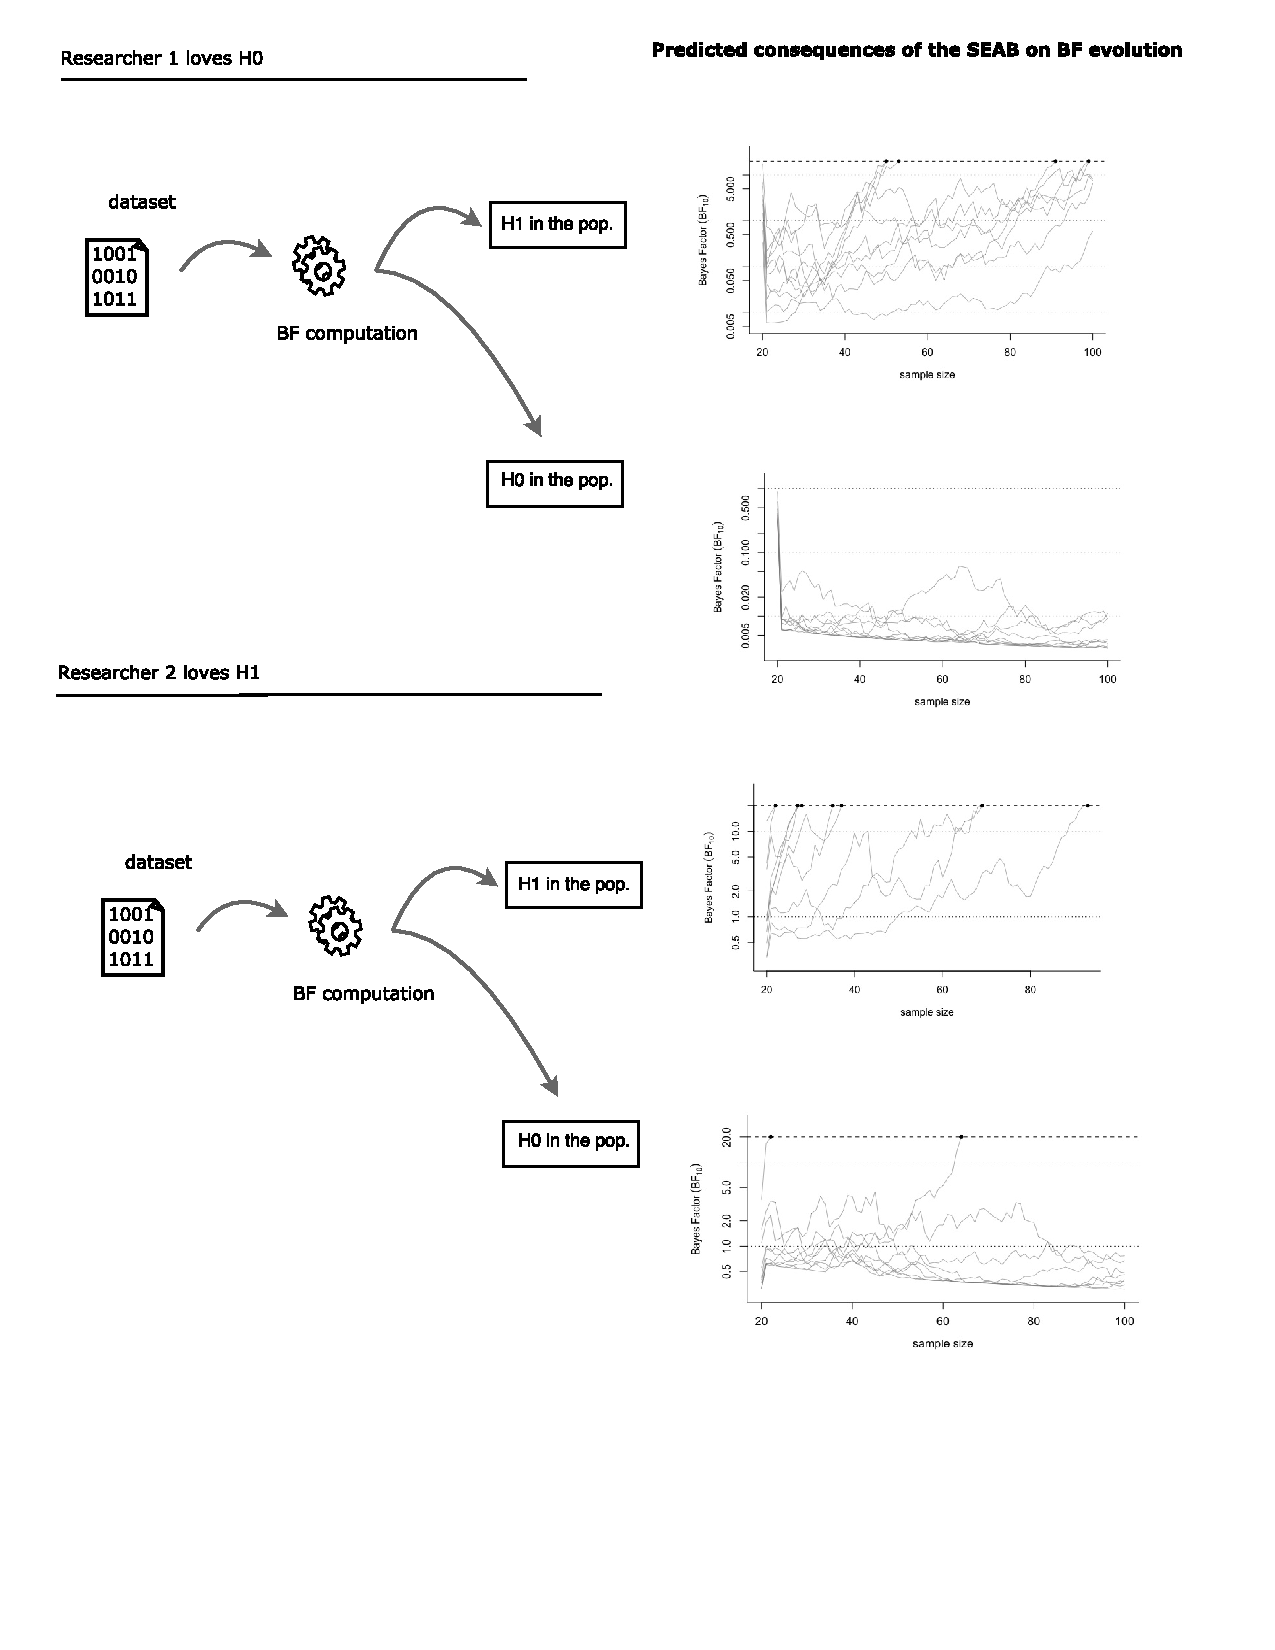
\includegraphics[width=1.1\textwidth]{figures/BFF_predictions.pdf}
%  \label{fig:pred}
%\end{figure*}

We have presented how the knowledge of previous data can bias the data collection process and have also illustrated the predicted consequences of these biases on the evolution of sequentially computed BFs. In the next section, we focus on how to prevent these biases from happening. We suggest two ways of implementing analysis blinding as a precaution against experimenter biases during sequential testing, and present a proof of concept for an automated procedure that would ensure objectivity.

\section{A fully automated, transparent, reproducible and triple-blind protocol for sequential testing}

Blinding is the procedure which hides the assigned condition from people involved in the experiment. It can notably be applied to participants, experimenters, or data analysts \citep{schulz_blinding_2002}. If possible, it is preferable to apply blinding to anyone involved in the experiment to avoid expectancy effects. Whereas participant and experimenter blinding is often considered in Psychology, much less attention has been given to analysis blinding, probably due to materials and time constraints. However, the use of analysis blinding would help eliminate some of the biases identified in \cite{wicherts_degrees_2016-1}. Again, this has been well described by \cite{lakens_performing_2014}: "In large medical trials, tasks such as data collection and statistical analysis are often assigned to different individuals, and it is considered good practice to have a data and safety monitoring board that is involved in planning the experiment and overseeing any interim analyses. In psychology, such a division of labor is rare, and it is much more common that researchers work in isolation".

Analysis blinding can take two different forms in the context of sequential analyses procedures. First, analysis blinding can refer to a procedure ensuring that the person analysing the data is blind to the hypotheses \citep{miller_blind_2011}. This configuration minimises intrapersonal biases because the analyst does not have the information necessary to influence data analysis in a specific direction (congruent or incongruent with the hypothesis). Second (and more specifically to sequential testing procedures), analysis blinding can refer to a procedure ensuring that the experimenter is blinded to the data analysis. This configuration minimises interpersonal biases because the experimenter does not have the information necessary to influence data collection in a specific direction (congruent or incongruent with the hypothesis).

If the experimenter is not the data analyst, they can be blind to the evolution of the intermediate results until data collection stops. As a consequence, the specific experimenter expectancy bias in the sequential procedure is avoided. Another solution is to automate analysis blinding so that the data analyst and the experimenter (who can be the same person) are blind to intermediate results computed on previous sets of observations. To illustrate this idea, we describe below how to perform transparent blind sequential analysis. We propose an example for two independent-groups comparisons \citep[as in][]{schonbrodt_sequential_2017}. This tutorial covers all experimental steps from preregistration to results reporting. When several options are available for a specific step, we detail one in the manuscript and other possibilities in the \hyperref[sec:supp]{\texttt{supplementary materials}}. We provide a functional example of the procedure on the OSF (Open Science Framework) based on an emotional Stroop experiment. In order to describe the procedure, we use the idea of \cite{rouder_what_2016} who took the perspective of his dog Kirby to explain Git and Github. Here we take the perspective of Lisa Loud,\footnote{\url{https://theloudhouse.fandom.com/wiki/Lisa\_Loud}} who loves carrying out experiments but has probably never used automated sequential analysis before.

\subsection{Prerequisites}

%Here are the main things Lisa needs to know or to do:

\begin{itemize}

\item Lisa needs to have an Open Science Framework (OSF, \url{https://osf.io/register/}) account.

\item Lisa needs to have at least some basic knowledge about how to use the OSF. See \cite{soderberg_using_2018} and \url{https://help.osf.io/} for a practical introduction.

\item Lisa needs to have \texttt{R} \citep{R-base} and RStudio (\url{https://www.rstudio.com/}) installed on her computer.

\item Lisa needs to have a recent version of OpenSesame (\url{https://osdoc.cogsci.nl/}) or PsychoPy (\url{https://www.PsychoPy.org/}) installed on her computer.

\end{itemize}

\subsection{"Born-open" data}

The aim of this this tutorial is not to discuss the theoretical work necessary before carrying out an experiment. We will directly focus on the preparation of materials needed to collect data. 

This tutorial mainly deals with computerised experiments.\footnote{However, some parts of the proposed protocol can be adapted to other kinds of experiments.} In this situation, users need to program an experiment to collect data. The logic proposed here is compatible with experiments programmed with PsychoPy \citep{peirce_PsychoPypsychophysics_2007,peirce_generating_2008,peirce_psychopy2_2019} or OpenSesame \citep{mathot_opensesame_2012}. These software programs have the advantage of being free and able to communicate with the OSF. These two qualities are crucial for transparent procedures and easy sharing. 

We will use the possibility to link the software program with the OSF in order to propose an intuitive "born-open" data procedure \citep{rouder_what_2016}. Although OSF synchronisation tools are generally easy to install on Windows and Mac OS, it can be slightly more "complicated" on other operating systems (OS) such as Linux OS. Most users probably work on Windows and Mac OS. However, because Linux OSs are free and open we believe that they fit well with the open science philosophy. Consequently, we will provide minimal examples on how to use this tutorial on Ubuntu as a popular and easy-to-use Linux distribution. \break

We propose a procedure using OpenSesame below. Procedures with PsychoPy can be found in the \hyperref[sec:supp]{\texttt{supplementary materials}}. OpenSesame probably allows the simplest synchronisation with the OSF. However, it is less flexible than PsychoPy for programming experiments because, unlike PsychoPy, it does not allow to access to a coder view. Direct OSF synchronisation is available with PsychoPy 2 but not with PsychoPy 3. The example available on the OSF is based on PsychoPy 2 but has also been successfully tested with OpenSesame. Table \ref{tab:soft} proposes a summary of the main strengths and weaknesses of each method.\\

\begin{table*}[t]
%\centering
\caption{Global overview of open experiment programming software's characteristics and synchronisation handling.}
\label{tab:softwares}
\resizebox{\textwidth}{!}{%
\begin{tabular}{@{}cccc@{}}
\toprule
 & \begin{tabular}[c]{@{}c@{}}OpenSesame\end{tabular} & \begin{tabular}[c]{@{}c@{}}PsychoPy 2\end{tabular} & \begin{tabular}[c]{@{}c@{}}PsychoPy 3\end{tabular} \\ \midrule
Synchronisation & OSF & OSF & Pavlovia and Gitlab* \\
Automatic synchronisation ease & + & - & - - - \\
Graphical interface for synchronisation & ++ & - & ++ \\
Synchronisation quality & ++ & + & +++ \\
Software flexibility & - & ++ & ++ \\ \bottomrule
\end{tabular}%
}
\vspace{1mm}
\begin{tablenotes}\footnotesize
\item[*] \textit{Indirect synchronisation is possible with OSF because synchronisation is possible between OSF and Gitlab. Direct synchronisation with OSF could also be possible but probably not straightforward.}
\end{tablenotes}
\label{tab:soft}
\end{table*}

\subsubsection{Programming the experiment for "born-open" data}

We present how to program an experiment allowing automatic "born-open" data with OpenSesame, currently the easiest way to program automatic "born-open" data. For more flexibility in experiment programming, PsychoPy options are described in the \hyperref[sec:supp]{\texttt{supplementary materials}}. OpenSesame is "a graphical experiment builder for the social sciences". It is free, open-source, and cross-platform. It features "a comprehensive and intuitive graphical user interface and supports Python scripting for complex tasks." \citep{mathot_opensesame_2012}. OSF integration is normally included by default for Windows and Mac OS. If not (or for other OS like Ubuntu for instance), the installation procedure is described in the \hyperref[sec:supp]{\texttt{supplementary materials}}. If OSF integration is installed, the user should see the OSF icon in OpenSesame (Figure \ref{fig:osfos}). Click the OSF log-in button and sign in with your OSF account. More details on OSF integration in OpenSesame can be found at \url{https://osdoc.cogsci.nl/3.1/manual/osf/}. If Lisa reads this part of the manual, she will know exactly what to do in order to link data to the OSF.\footnote{The following part is a reformulation of the manual for the purpose of our tutorial.} If she links data to the OSF, each time that data has been collected (normally after every experimental session), this data is also uploaded to the OSF. Lisa should follow the following steps in order to do so:

\begin{itemize}
    \item Lisa has to save the experiment on her computer.
    \item She then has to open the OSF explorer, right-click on the folder that she wants the data to be uploaded to, and select "Sync data to this folder". The OSF node that the data is linked to will be shown at the top of the explorer.
    \item She finally needs to check "Always upload collected data" and data files will be automatically saved to OSF after they have been collected. 
\end{itemize}

\begin{figure}[H]
  \caption{OSF log-in button in the main toolbar in OpenSesame}
  \centering
  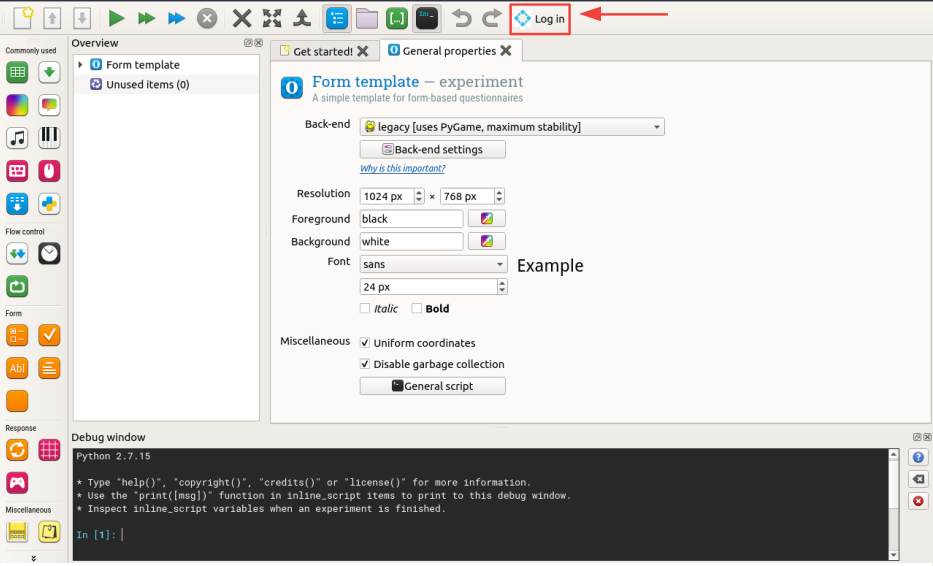
\includegraphics[width=0.5\textwidth]{figures/osf_logo_opensesame_red.png}
  \label{fig:osfos}
\end{figure}

\subsection{Script preparation and piloting}

Performing sequential analyses requires strict experiment programming and data analysis preparation. Because data is continuously analysed during data collection, everything must be ready before collecting data. This can be seen as a disadvantage because there is a lot of work to be done before data collection. Indeed, analysing data after data collection allows us to delay several choices thus allowing to launch data collection more quickly.\footnote{Here we do not say that preparation is specific to sequential testing. Preparation can be recommended for all designs, but is not avoidable in sequential analysis.} However, this can also be considered as a huge advantage because there are no unexpected surprises after data collection. It is not possible to discover that something has not been recorded or that data is not in the appropriate format, or that data is more difficult to analyse than expected. Everything is thought about upstream because everything must work for data analysis which is performed during data collection. We propose this 6-step procedure to prepare the analysis:

\begin{itemize}
    \item Clearly define the variables involved in the study in order to program the experiment
    \item Carefully consider how to analyse the data to be collected
    \item Program the experiment in keeping with the planned data analysis
    \item Test the experiment to check that everything is working as expected
    \item Prepare the scripts that will be used to analyse data
    \item Run some pilots to test the procedure
\end{itemize}

These steps are necessary in order to launch the actual experiment. Otherwise, sequential analyses are likely to fail at some point.

\subsection{Preregistration}

Let's assume Lisa has successfully achieved script preparation and piloting. When everything is ready, she has everything she needs to preregister her study. Preregistration is very important in sequential testing because it forces Lisa to explicitly state her statistical criteria of interest and therefore announce when data collection will end. This is very useful in order to limit biases due to Lisa's degrees of freedom \citep{lakens_performing_2014,wicherts_degrees_2016-1}.

In addition to generic preregistration, the first important thing to preregister is the sequential data cleaning procedure. In this part, Lisa should describe how data will be handled before inferential statistical modelling. This can include, physiological signal processing, potential observation or participant removal criteria or any other data manipulation happening between data collection and modelling. After that, Lisa should indicate the appropriate stopping statistics depending on the procedure (e.g., SBF, HDI+ROPE, precision). The stopping statistic should be described along with a clear and detailed description of the model which is computed to get this statistic. Finally, Lisa should also specify a minimum sample size required to compute the models, and a maximal sample size affordable for her, which would determine the end of data collection, independently of the stopping statistic.

\subsection{Transparent data collection}

When possible, making data openly available can improve the quality of science \citep{klein_practical_2018}. In the context of sequential data analysis, it can be even more important. As we explained above, sequential analyses offer strong advantages but also increase Lisa's degrees of freedom. Making data open can reduce this bias. In this perspective, born open data \citep{rouder_what_2016} can be even more efficient, especially in the context of sequential analysis. "Born-open" data is the procedure which makes data automatically open as soon as it is collected. This procedure has at least two huge interests for sequential analysis. First, the time course of data collection is transparent because data is necessarily sent online and time-stamped just after being collected. This is very important because in doing so, each choice made by Lisa will be clear and justified. Second, "born-open" data will facilitate real time online data analysis which is very useful for sequential designs. automatic "born-open" data is possible with OpenSesame or PsychoPy by automatic publishing data on the OSF (or on Github or Gitlab for instance).

\subsection{Automated data cleaning}

After collecting her first batch of data, Lisa might not be able to directly fit the statistical model she is interested in. She probably needs a procedure of data cleaning in order to get her data ready for statistical inference. Data cleaning can include physiological signal processing, artefacts removal, errors removal, dealing with potential outliers, and everything needed to get meaningful data from raw data. Lisa has to perform data cleaning before statistical modelling. Because Lisa is analysing data sequentially, she also has to clean data sequentially.

For instance, in our example (the emotional Stroop task), we decided to remove missing data and response times (RT) below 100 ms. This is done each time new data is incorporated (see lines 101 to 110 of the \texttt{sequential$\_$analyses.R} script). We could also have chosen to analyse RT only for correct responses and/or to remove observations based on a specific descriptive statistic.

\subsection{Automated blind data analysis}

Because Lisa has prepared everything needed for her procedure, she is able to automate data analysis and therefore to be blind to the details of the analysis while she is collecting data. Here is how she can proceed and how we proceeded in our example.

We describe how Lisa can handle tasks-scheduling on a UNIX system (macOS and Linux) in this paragraph. Lisa can use the \texttt{cronR} package \citep{Wijffels_cronR_2018} to schedule tasks in \texttt{R}. This package will be useful in order to retrieve data from the OSF and to analyse it. Lisa will have to create a task by running the appropriate script (\texttt{main\_script.R} in our example) once before collecting the first observation. She will be able to decide how often she wants the script to run automatically. Lisa could also apply the same procedure on a Windows system thanks to the \texttt{taskscheduleR} package \citep{Wijffels_taskscheduleR_2018}. A short description on how to use this package can be found at: \url{https://cran.r-project.org/web/packages/taskscheduleR/vignettes/taskscheduleR.html}.

If Lisa chooses that the script should auto-run each hour, the main script will check data from the OSF each hour. This will be done with the \texttt{osfr} package \citep{wolen_osfr_2019}. In our example (Line 106 to 143 in \texttt{main\_script.R}), we check if new data is available on the OSF and download it if it is the case. 
After a little bit of data formatting (lines 145 to 183), the script will run the sequential analysis (line 218 to 263). The main script calls the \texttt{sequential\_analyses.R} script which contains the sequential analyses function. Lisa will also have to specify some parameters depending on the model she is interested in.

At the end of the analysis, Lisa will receive an e-mail (line 265 to 283) telling her whether to stop or to continue data collection. This em-mail will neither report the effect nor its direction, but only the information to stop or to continue the data collection. This means that Lisa will be able to follow a sequential design without any information about the results of data analysis, excepted the fact that she has (not) reached her criterion. The mail will be sent automatically in \texttt{R} thanks to the \texttt{gmailR} package \citep{hester_gmailr_2016}.

\subsection{Reproducible reporting}

Lisa will stop data collection when she reaches her statistical criterion or her maximum affordable sample size. She will then be able to write a report describing her results. She can do it using RMarkdown \citep{Allaire_rmarkdown_2019,Xie_RMarkdown_2018} in order to incorporate her results automatically from her R scripts into her report \citep[e.g., see][]{bauer_writing_2018}. Lisa could for instance use the \texttt{R} package \texttt{papaja} \citep{Aust_papaja_2018} which would allow her to write a reproducible APA manuscript with RMarkdown. Scientific writing with Rmarkdown has important benefits for any type of research design but would be even more valuable for sequential analyses.

\subsection{Feasibility of the proposed protocol and limitations}

A graphical summary of the procedure is depicted in Figure \ref{fig:safeseqan}.\footnote{This figure has been inspired by the Figure 1 in \cite{quintana_guidelines_2016}.} All the tools needed to set it up are available for free to everyone. Using OpenSesame or PsychoPy is relatively straightforward and does not necessarily require coding skills. We proposed standard \texttt{R} scripts in order to automate sequential analysis. However, we concede that using this scripts requires minimal knowledge of \texttt{R}. Hence, we also propose a Shiny application available at \url{https://barelysignificant.shinyapps.io/blind_sequential_analyses/}. With this application, Lisa would just have to specify all the important details of her analysis in boxes, from which the application generates the corresponding \texttt{R} script almost ready for sequential analysis. This application is meant to facilitate the creation of \texttt{R} scripts. It automatically writes around 90\% of the code Lisa would have to write to use such a sequential analysis procedure. However, it is almost certain that the produced \texttt{R} code would not work immediately. It would require some minor tweaking from her, such as checking the local path, making sure that the scripts and the data are in the same repository, adapting the data import step to specific properties of the data under consideration, and so on.

The procedure proposed here only requires one computer. Hence, the implementation cost is rather low. This procedure is also well suited for multi-lab studies. Indeed, an experiment can be run at different places but data is automatically centralised on one platform  and can be analyse automatically and sequentially by one single computer. The experiment we designed with PsychoPy 2 (see the supplementary material for more information) is specifically thought for multi-lab studies by automatically recording information about the computer which runs the experiment. This enables the identification of the site associated with each participant. 

We concede that automation of data analysis prevents one interesting advantage of sequential testing. Namely, the fact that data collection can be stopped whenever the behaviour of data is unexpected, allowing the experimenter to rethink the experimental design or aim before collecting more data \citep{lakens_performing_2014}. Depending on the confidence and expected familiarity with the data to be collected, the researchers have to choose between automated or "two-person" analysis blinding. The first option has low costs of implementation whereas the second one is more flexible. In any case, after performing a sequential analysis, nothing prevents Lisa from performing additional analyses based on unexpected data specificity, taking care to record and state the exploratory nature of any such analyses.

\begin{figure}[H]
  \caption{Schematic procedure of a transparent and blind sequential data analysis.}
  \centering
  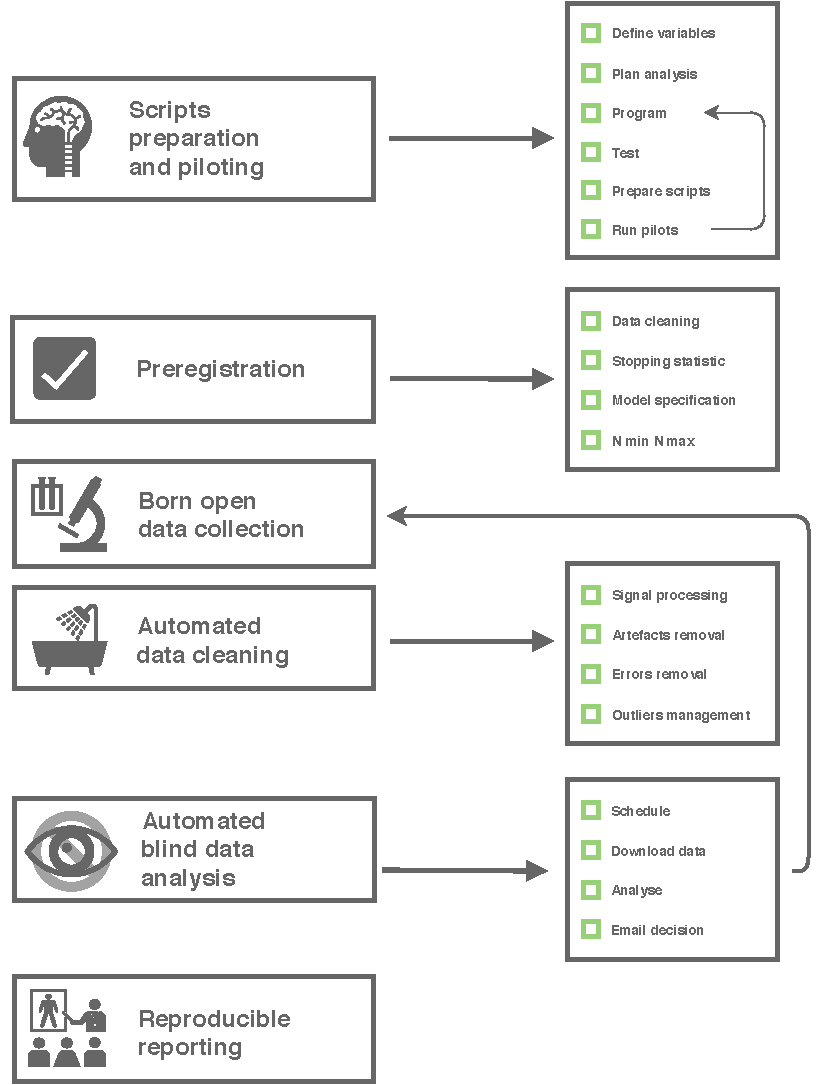
\includegraphics[width=0.49\textwidth]{figures/safeseqan.pdf}
  \label{fig:safeseqan}
\end{figure}

\subsection{A word on blind analysis by multiple people}

If Lisa can afford working with a colleague on her study and if she prefers to do so, we advise her to apply the logic of the automated procedure described in this tutorial. The only difference will be that her colleague will analyse data while Lisa collects it (or conversely). If her colleague analyses data, they will have to retrieve data online (e.g., on OSF) and to perform the planned preregistered analysis (unless data behave very unexpectedly in which case they will have the responsibility to adapt the analysis or stop data collection prematurely). The only contact Lisa and her colleague will have concerning the experiment will be the email they will send to inform Lisa whether to stop or continue data collection, nothing more.

\section{Conclusions}

We began by presenting the intra and interpersonal biases that might emerge during sequential testing and sequential analysis procedures. To tackle these issues, we proposed a novel automated, transparent, reproducible and blind protocol for sequential analysis. The main interest of this procedure is to reduce possible biases that could be encountered during intermediate data analysis and to prevent the inflation of social influences during data collection.

This protocol should be considered as a proof-of-concept for sequential analysis automation. However, future work will be able to propose more comprehensive and more user-friendly solutions for sequential analyses. For instance, the reliance on the user's \texttt{R} programming skills might be alleviated with the development of an online platform that would automate the procedure online, without the need for coding.

More work is also needed to precisely quantify intra and interpersonal biases during data collection and analysis. For instance, one could set up experimental procedures to pinpoint these biases in realistic lab situations \citep [e.g., see][]{gilder_role_2018}. In addition to experimental procedures, computational modelling could also be used to estimate the presence of bias in extant (published or not) sequential analyses. By formalising the sequential analysis procedure (e.g., using an evidence accumulation model) and by explicitly modelling the biases that we describe in the present article, we might be able to assess the likelihood that an observed set of collected statistics (e.g., BFs) has been obtained under the assumption of bias (or no bias).

\section{Supplementary materials}\label{sec:supp}

Reproducible code and supplementary materials are available on OSF: \href{https://osf.io/mwtvk}{\nolinkurl{https://osf.io/mwtvk/}}.

\section{Acknowledgements}

We thank Hans IJzerman for helpful comments and Edward Collett for his help with manuscript English proof reading on a previous version of this manuscript. Many thanks to Christopher Moulin for his feedback and for his help with manuscript English proof reading on the updated version of this manuscript. We also thank Rickard Carlsson, Félix Schönbrodt, Angelika Stefan, Stephen Martin, and Charlotte Brand for insightful comments and suggestions during the peer-review process.

\bibliography{BBF}

\end{document}
